\section{Features}

When doing speaker recognition it is advantageous to classify on the basis of extracted features from speech data, rather than the audio samples themselves. \ref{} % Reference
Therefore some features ware extracted, using the following techniques before further processing.

\section{Mel-frequency Cepstral Coefficients}
In this project, the features used for classification are based on Mel-frequency Cepstral Coefficients (MFCC).
They have proven effective for use in speaker recognition, in other implementations. \ref{} % Reference

A mel-frequency cepstrum is dscribed as a cepstrum (a nonlinear spectrum-of-a-spectrum) on a mel-frequency scale.
The mel-scale is a non-linear frequency scale that mimics the characteristics of the human ear.
It is approximately linear below $ 1000\ Hz $ and logarithmic above.
This makes it ideal for audio and human speech processing.

Besides the bare MFCCs, the $ 0^{th} $ order coefficients, which are equivalent to the energy, and the delta and double-delta coefficients, which are the temporal derivatives $ \frac{dc}{dt} $ and double-derivatives $\frac{d^2c}{dt}$ respectively, are used as features.


\section{Feature extraction}
\subsection{Framing}
In this project we have chosen a to segment data into short frames, and extract features for classification on the basis of these.
We have chosen a frame length of $ 256\ samples $ with a spacing of $ 100\ samples $.

This means that we have a frame length of
\begin{equation}
t_{frame length} = \dfrac{N_{frame}}{F_s} = \dfrac{256}{48\ kHz} = 5.33\ ms
\end{equation}

and a frame interval of
\begin{equation}
t_{frame interval} = \dfrac{N_{interval}}{F_s} = \dfrac{100}{48\ kHz} = 2.08\ ms
\end{equation}
\newpage
\subsection{MFCC feature calculation}
The extraction of MFCC features from audio samples is done in MATLAB, using an open-source toolbox called Voicebox.
It calculates the MFCCs in the following way: (See Figure \ref{fig:mfccFlow})

\begin{figure}[H]
\centering
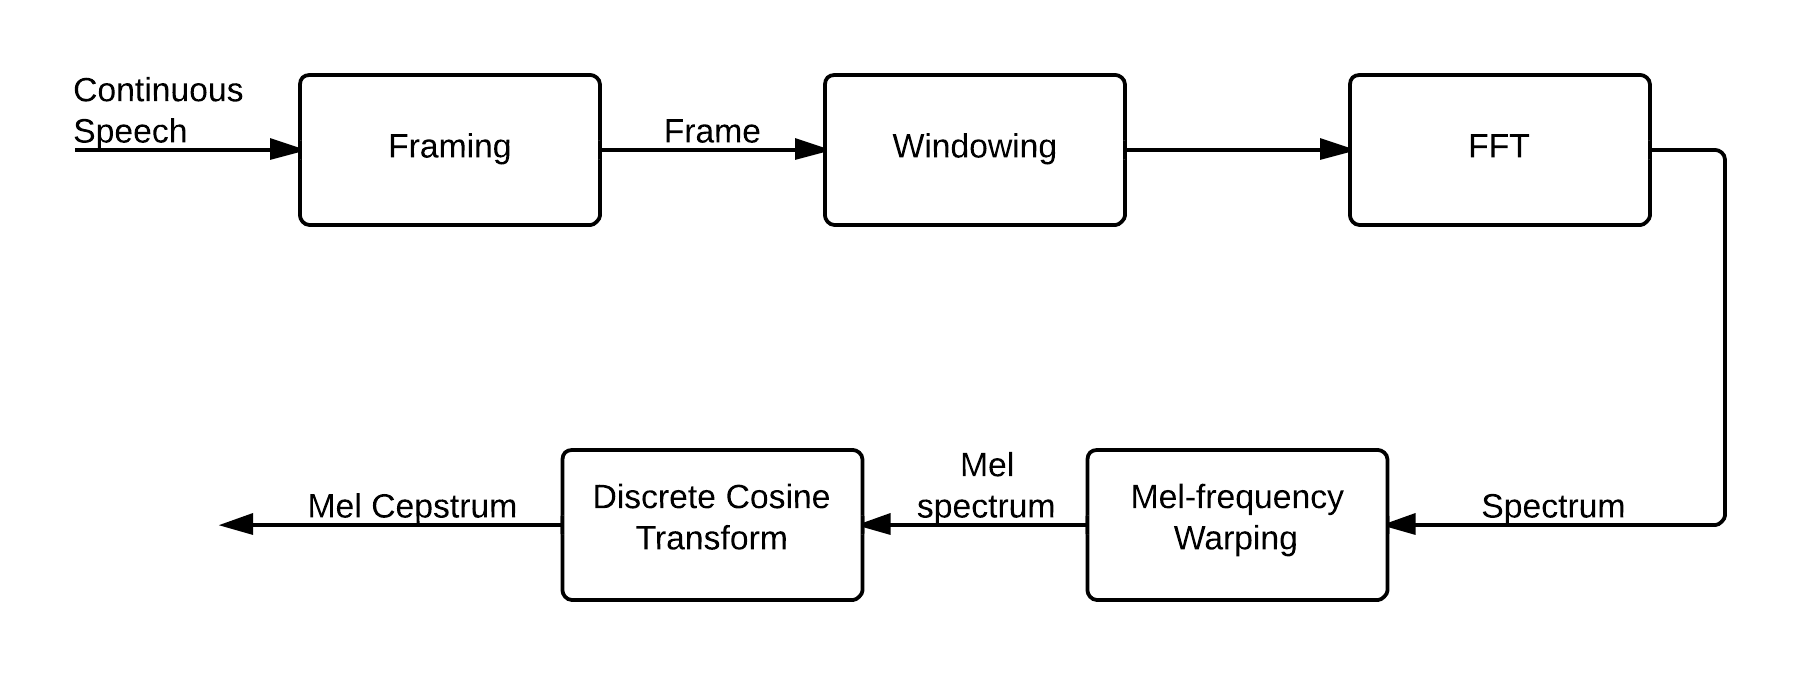
\includegraphics[width=0.8\linewidth]{MFCC_Flowchart_PNG}
\caption{Flowchart of MFCC calculation}
\label{fig:mfccFlow}
\end{figure}

\begin{enumerate}

\item
The current frame is windowed with a Hamming window.

\item
The frame is Fourier transformed.

\item
The power of the spectrum is mapped to a mel-scale, using triangular overlapping windows. (See Figure \ref{fig:mfccBank})

\item
Take the logarithm of the power a each mel-frequency

\item
Take the Discrete Cosine Transform (DCT) of the log-powers as is it were a signal.

\item
The MFCCs are the amplitudes of the resulting spectrum.

\end{enumerate}

\begin{figure}[H]
\centering
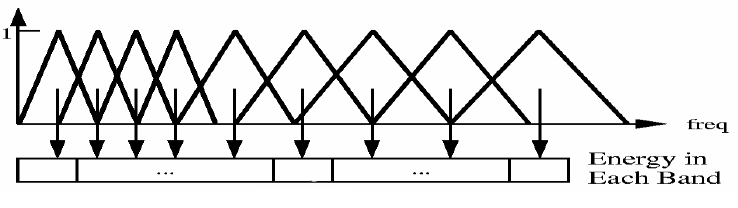
\includegraphics[width=0.8\linewidth]{MFCC-bank}
\caption{an example of a mel-spaced filterbank}
\label{fig:mfccBank}
\end{figure}
